\documentclass[a4paper,11pt]{article}

\usepackage[T1]{fontenc}
\usepackage[utf8]{inputenc}
\usepackage{graphicx}
\usepackage{xcolor}
\usepackage{caption}
\usepackage{subcaption}

\usepackage{tgtermes}

\usepackage[
pdftitle={Statistical Machine Learning}, 
pdfauthor={Inez Wijnands \& Guido Zuidhof, Radboud University Nijmegen},
colorlinks=true,linkcolor=blue,urlcolor=blue,citecolor=blue,bookmarks=true,
bookmarksopenlevel=2]{hyperref}
\usepackage{amsmath,amssymb,amsthm,textcomp}
\usepackage{enumerate}
\usepackage{multicol}
\usepackage{tikz}

\usepackage{geometry}
\geometry{total={210mm,297mm},
left=25mm,right=25mm,%
bindingoffset=0mm, top=20mm,bottom=20mm}


\linespread{1.3}

\newcommand{\linia}{\rule{\linewidth}{0.5pt}}

% custom theorems if needed
\newtheoremstyle{mytheor}
    {1ex}{1ex}{\normalfont}{0pt}{\scshape}{.}{1ex}
    {{\thmname{#1 }}{\thmnumber{#2}}{\thmnote{ (#3)}}}

\theoremstyle{mytheor}
\newtheorem{defi}{Definition}

% my own titles
\makeatletter
\renewcommand{\maketitle}{
\begin{center}
\vspace{2ex}
{\huge \textsc{\@title}}
\vspace{1ex}
\\
\linia\\
\@author  \@date
\vspace{4ex}
\end{center}
}
\makeatother
%%%

% custom footers and headers
\usepackage{fancyhdr,lastpage}
\pagestyle{fancy}
\lhead{}
\chead{}
\rhead{}
\lfoot{Assignment \textnumero{} 1}
\cfoot{}
\rfoot{Page \thepage\ /\ \pageref*{LastPage}}
\renewcommand{\headrulewidth}{0pt}
\renewcommand{\footrulewidth}{0pt}
%

% code listing settings
\usepackage{listings}
\lstset{
    language=Python,
    basicstyle=\ttfamily\small,
    aboveskip={1.0\baselineskip},
    belowskip={1.0\baselineskip},
    columns=fixed,
    extendedchars=true,
    breaklines=true,
    tabsize=4,
    prebreak=\raisebox{0ex}[0ex][0ex]{\ensuremath{\hookleftarrow}},
    frame=lines,
    showtabs=false,
    showspaces=false,
    showstringspaces=false,
    keywordstyle=\color[rgb]{0.627,0.126,0.941},
    commentstyle=\color[rgb]{0.133,0.545,0.133},
    stringstyle=\color[rgb]{01,0,0},
    numbers=left,
    numberstyle=\scriptsize\ttfamily,
    stepnumber=1,
    numbersep=10pt,
    captionpos=t,
    escapeinside={\%*}{*)}
}

%%%----------%%%----------%%%----------%%%----------%%%

\begin{document}

\title{Statistical Machine Learning \\ Assignment 1}

\author{Inez Wijnands (s4149696) \& Guido Zuidhof (s4160703)\\ Radboud University Nijmegen\\}

\date{29/09/2015}

\maketitle

\noindent \textit{The entire code listing is in a separate file. The listings shown here are merely code snippets}.\vspace{-0.5cm}
\section*{Exercise 1}
\begin{enumerate}
	\item The function $t = f(x)$ we have created is $f(x) = 1 + sin(8x+1)$. This function is neither even nor odd. An even function is a function such as $cos(x)$, and an odd function is a function such as $sin(x)$, since we changed the phase and intercept of $sin(x)$ our function is neither. See Figure 1 for the function $f(x)$ and observations $\mathcal{D}$. \vspace{-0.2cm}
		\begin{figure}[h]
			\centering
			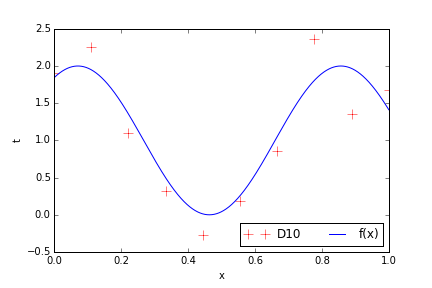
\includegraphics[scale=0.8]{1_1.png}\vspace{-0.5cm}
			\caption{\vspace{-0.2cm}The function $f(x)$ and observations $\mathcal{D}$ are plotted (similar to Bishop, Fig.1.2)}
		\end{figure}
	\item See Listing 1 for the function $\boldsymbol{w} = PolCurFit(\mathcal{D},M)$.\vspace{-0.5cm}
		\begin{lstlisting}[label={list:first},caption=Python code for function PolCurFit -- Input are the observations $\mathcal{D}$ and the results $t$ of function $f(x)$ and the order of the polynomial $M$. The functions calculates the $A$-matrix and $T$-vector and solves this equation to find the weights.]
def PolCurFit(D,M):
    x = D[0]
    t = D[1]
    M = M + 1
    A = np.array([[Aij(i,j,x) for j in xrange(M)] for i in xrange(M)])
    T = np.array([Ti(i,t,x) for i in xrange(M)])
    return np.linalg.solve(A,T)
		\end{lstlisting}
	\item See Figure 2 \& 3 \vspace{-0.2cm}
		\begin{figure}[h]
			\centering
			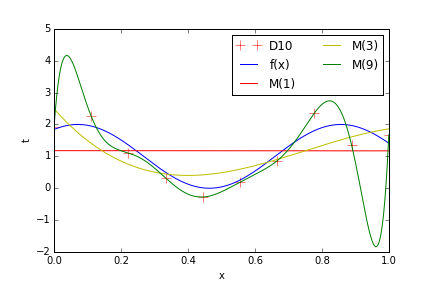
\includegraphics[scale=0.8]{1_2_10.png}\vspace{-0.5cm}
			\caption{\vspace{-0.2cm} In this figure, the observations $\mathcal{D}$, the function $f(x)$ and polynomials of different orders of $M$ are shown.}
		\end{figure}
		\vspace{-0.5cm}
		\begin{figure}[h]
			\centering
			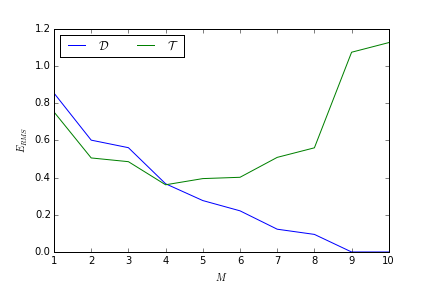
\includegraphics[scale=0.8]{1_3_10.png}\vspace{-0.5cm}
			\caption{\vspace{-0.2cm} For the various orders $M = [1,\hdots,10]$ and for each solution $\boldsymbol{w}^*$ the root-mean-quare error $E_{RMS} = \sqrt{2E(\boldsymbol{w}^*)/N}$ is computed of the corresponding polynomial, evaluated on both the training set $\mathcal{D}$ and the testset $\mathcal{T}$ (similar to Bishop, Fig.1.5)}
		\end{figure}\vspace{-0.5cm}
	\item See Figure 4 \& 5.
		\begin{figure}[h!]
			\centering
			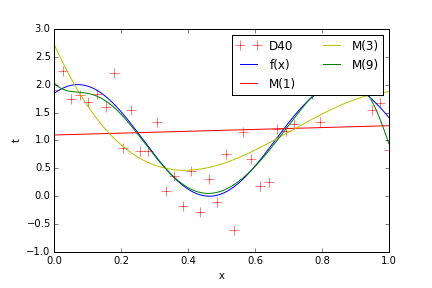
\includegraphics[scale=0.8]{1_2_40.png}\vspace{-0.5cm}
			\caption{\vspace{-0.2cm} In this figure, the observations $\mathcal{D}$, the function $f(x)$ and polynomials of different orders of $M$ are shown.}
		\end{figure}
		\begin{figure}[h!]
			\centering
			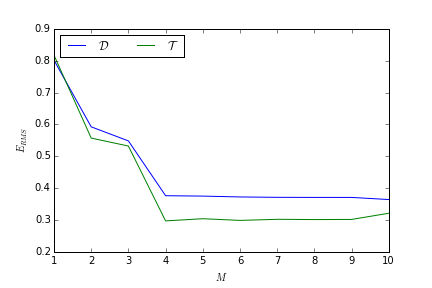
\includegraphics[scale=0.8]{1_3_40.png}\vspace{-0.5cm}
			\caption{\vspace{-0.2cm} For the various orders $M = [1,\hdots,10]$ and for each solution $\boldsymbol{w}^*$ the root-mean-quare error $E_{RMS} = \sqrt{2E(\boldsymbol{w}^*)/N}$ is computed of the corresponding polynomial, evaluated on both the training set $\mathcal{D}$ and the testset $\mathcal{T}$. (similar to Bishop, Fig.1.5)}
		\end{figure}
		Since there are now 40 observations in $\mathcal{D}$, larger order polynomials work better. For 10 observations, a polynomial of the 10th order will create a function that goes straight through every observation, as you can see in Figure 2, but these observations are noisy, thus the function $f(x)$ will not be found, and adding more observations will cause the error to increase dramatically since these will not follow the curves of that polynomial. With more observations, the 9th- and 10th-order polynomials do not match every observation, but it will be a far better approximation of $f(x)$. In Figure 3 and 5, you can see that when the order is the same as the amount of observations the error can become zero, but a change in the order will increase the error drastically. With more observations in the training set, the error of the training set and testset are more similar. 
	\item We included the $\lambda$ parameter in the $A$-matrix. Since the gradient of \textit{\~{E}} with respect to $\boldsymbol{w}$ is $A\boldsymbol{w}-\boldsymbol{T} + \lambda \boldsymbol{w}$, we can rewrite this to $(A+\lambda I)\boldsymbol{w} - \boldsymbol{T}$ \footnote{See Bishop, pp.144-145 for the used theory behind the regularization of the least-squares, using $\lambda$ with the identity matrix.} See Listing 2 for the altered function $PolCurFit()$. See Figure 6 and 7 for the results of the modified $PolCurFit()$.
		\begin{lstlisting}[label={list:second},caption=Python code for function PolCurFit -- Penalty added.]
def PolCurFit(D,M, _lambda=0):
    x = D[0]
    t = D[1]
    M = M + 1
    
    #Construct A matrix by calling Aij function for every entry
    A = np.array([[Aij(i,j,x) for j in xrange(M)] for i in xrange(M)])
    
    #Ridge Regression
    A = A + _lambda * np.identity(len(A))    
    
    #Construct T vector
    T = np.array([Ti(i,t,x) for i in xrange(M)])
    return np.linalg.solve(A,T)
		\end{lstlisting}

		\begin{figure}[h!]
			\centering
			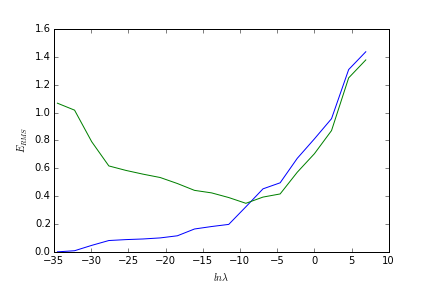
\includegraphics[scale=0.8]{1_5.png}\vspace{-0.5cm}
			\caption{For $M = 9$, we calculated the root-mean-squared error for the training set $\mathcal{D}$ and the testset $\mathcal{T}$. You can see that the root-mean-squared error increases for larger $\lambda$ for $\mathcal{D}$ and first decreases and later increases for $\mathcal{T}$. You try to minimize both the error and the sum of the weights, and these weights are regularized by $\lambda$. If your $\lambda$ is very high, the weights become smaller to minimize the sum of the error plus the $\lambda$ times the weights. For a large order polynomial (such as $M = 9$ as in this plot, the weights have to be quite high to pass all the data points in the training set as close as possible. This is however noisy data, with few observations. But for larger $\lambda$, you lower the weights, and thus the error will increase. (similar to Bishop, Fig.1.8)}
		\end{figure}
		\begin{figure}[h!]
			\centering
			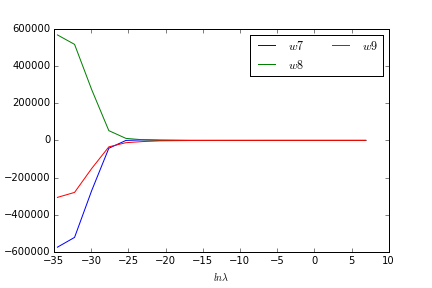
\includegraphics[scale=0.8]{1_5_2.png}\vspace{-0.5cm}
			\caption{The value of the weights of the 7th-, 8th- and 9th-order polynomials are plotted against the regularizer $\lambda$. You can see that the weights are driven to zero. }
		\end{figure}

\end{enumerate}

\pagebreak
\section*{Exercise 2}
\begin{enumerate}
	\item \begin{figure}[h!]
   			\centering
   			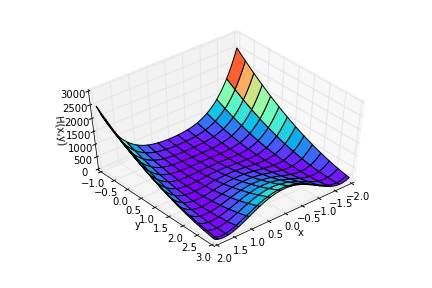
\includegraphics{surfaceplot.png}\vspace{-0.5cm}
   			\caption{\vspace{-0.2cm} Surface plot of $h(x,y)$ over the interval $[-2\leq x \leq 2] \times [-1 \leq y \leq 3]$.}
  		\end{figure}
 
		\noindent At first glance the function seems symmetrical, but it's not. The gradient is very small in the \emph{valley} visible in the plot, it does however only have 1 minimum and no local minima (at least in this interval).
We expect convergence to be fairly slow due to this low gradient.
	\item First we rewrite $h(x,y)$:\\
		$h(x,y) = 100(y - x^2)^2 + (1 - x)^2 = 100(y^2 - 2x^2y + x^4) + x^2 - 2x + 1 =$ \\
		$100y^2 - 200x^2y + 100x^4 + x^2 - 2x + 1$\\
		\\
		We compute the gradient of $h(x,y)$ with respect to $x$ and with respect to $y$:\\
		$\frac{dh(x,y)}{dx} = - 400xy + 400x^3 + 2x - 2$\\
		$\frac{dh(x,y)}{dy} = 200y - 200x^2$\\
		\\
		Set derivative of $h(x,y)$ equal to zero to find minimum:\\
		$200y - 200x^2 = 0 \rightarrow 200y = 200x^2 \rightarrow y = x^2$\\
		$- 400xy + 400x^3 + 2x - 2 = 0 \rightarrow$ use $y = x^2$ $\rightarrow 400x^3 = 400x^3 + 2x - 2 \rightarrow 			2x = 2 \rightarrow x = 1$\\
		$y = x^2$ and $x = 1 \rightarrow y = 1^2 = 1$\\
		(1,1) is the minimum of $h(x,y)$
	\item Gradient descent iteration rule:\\
		$x_{n+1} = x_n - \eta \nabla E(x_n)$\\
		$E(x_n) = h(x,y)$\\
		\\
		$x_{n+1} = x_n - \eta \frac{dh(x_n,y_n)}{dx_n} = x_n - \eta(- 400x_ny + 400x_n^3 + 2x_n - 2$\\
		$= (1 + \eta 400y) * x_n - \eta 400x_n^3 - \eta 2x_n + \eta 2$\\
		$= (\eta 400y - 1)x_n - \eta 400x_n^3 + \eta 2$\\
		\\
		$y_{n+1} = y_n - \eta \frac{dh(x_n,y_n)}{dy_n} = y_n - \eta(200y_n - 200x^2)$\\
		$= (1 - \eta 200)y_n - \eta 200x^2$
	\item We investigated $\eta \in \{0.01, 0.001, 0.0001, 0.00001\}$, as starting point we took $(-2,2)$. $\eta = 0.01$ did not converge, as the steps it took were large enough to end up higher on the opposite side of the valley. It quickly moved out of bounds. The other values of $\eta$ did converge, see Table \ref{conver} for the number of iterations for the specific amount of iterations required. A smaller value of $\eta$ leads to a higher amount of iterations required, as was expected. The $\eta$ parameter can not be too high, as it would quickly go out of bounds when started on the steep gradient found at the edge of the interval.\\
		\\
		The very low gradient and the relatively low $\eta$ required makes for very slow numerical minimization with gradient descent for this function. See below for the trajectory plots.
 
		\begin{table}[h!]
			\centering
			\caption{Convergence of GD for different values of $\eta$}
			\label{conver}
			\begin{tabular}{p{2cm} | p{4.5cm}}
				$\eta$    & Iterations until convergence \\ \hline
				0.01    & Did not converge             \\
				0.001   & 26390                        \\
				0.0001  & 267391                       \\
				0.00001 & 2674138               
			\end{tabular}
		\end{table}\vspace{-0.5cm}
 
		\begin{figure}[h!]
			 \centering
   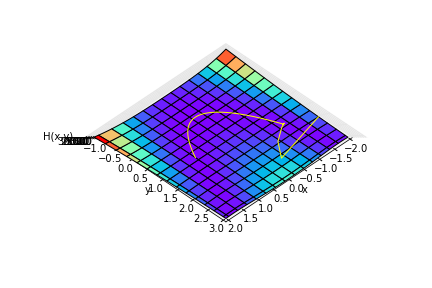
\includegraphics{trajectory0001y26390}\vspace{-0.5cm}
   \caption{\vspace{-0.2cm} Trajectory of gradient descent with $\eta = 0.001$.}
  \end{figure}\vspace{-0.5cm}
 
\begin{figure}[h!]
   \centering
   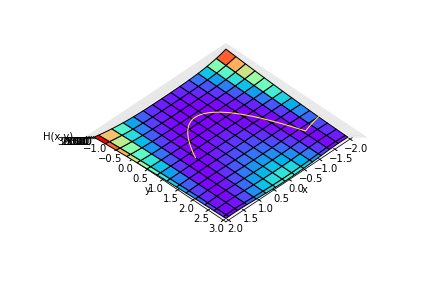
\includegraphics{trajectory00001y267391}\vspace{-0.5cm}
   \caption{\vspace{-0.2cm} Trajectory of gradient descent with $\eta = 0.0001$.}
  \end{figure}\vspace{-0.5cm}
 
\begin{figure}[h!]
   \centering
   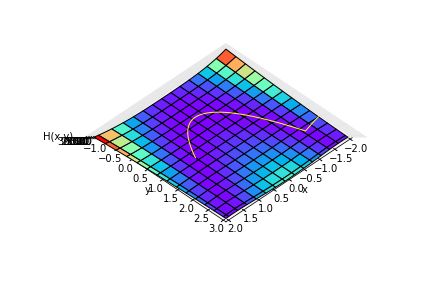
\includegraphics{trajectory1e-05y2674138}\vspace{-0.5cm}
   \caption{\vspace{-0.2cm} Trajectory of gradient descent with $\eta = 0.00001$.}
  \end{figure}
\end{enumerate}

\pagebreak
\section*{Exercise 3}
\begin{enumerate}
\item Initial probability of grabbing an apple:\\
$P(F_1 == Apple) =$\\
$P(B == 1) * P(F_1 == Apple | B == 1) + P(B == 2) * P(F_1 == Apple | B == 2)$ \\
$= \frac{1}{2} * \frac{8}{12} + \frac{1}{2} * \frac{15}{18}$ \\
$= \frac{4}{12} + \frac{15}{36} = \frac{27}{36} = \frac{3}{4}$\\
\\
Initial probability of grabbing a grapefruit:\\
$P(F_2 == Grapefruit) = $\\
$P(B == 1) * P(F_2 == Grapefruit | B == 1) + P(B == 2) * P(F_2 == Grapefruit | B == 2)$ \\
$= \frac{1}{2} * \frac{4}{12} + \frac{1}{2} * \frac{3}{18}$ \\
$= \frac{2}{12} + \frac{3}{36} = \frac{1}{4}$\\
\\
Probability of having grabbed from box 1 given that you grabbed a grapefruit:\\
$P(B == 1 | F_2 == Grapefruit) = \frac{P(F_2 == Grapefruit | B == 1) * P(B == 1)}{P(F_2 == Grapefruit)}$\\
$= \frac{\frac{4}{12} * \frac{1}{2}}{\frac{1}{4}}$\\
$= \frac{\frac{2}{12}}{\frac{1}{4}} = \frac{8}{12} = \frac{2}{3}$\\
\\
Probability of having grabbed from box 2 given that you grabbed a grapefruit:\\
$P(B == 2 | F_2 == Grapefruit) = \frac{P(F_2 == Grapefruit | B == 2) * P(B == 2)}{P(F_2 == Grapefruit)}$\\
$= \frac{\frac{3}{18} * \frac{1}{2}}{\frac{1}{4}}$\\
$= \frac{\frac{3}{36}}{\frac{1}{4}} = \frac{12}{36} = \frac{1}{3}$\\
\\
Probability of grabbing an apple but with updated probabilities for the boxes since these are given having grabbed a grapefruit:\\
$P(F_1 == Apple) = $\\
$P(B == 1) * P(F_1 == Apple | B == 1) + P(B == 2) * P(F_1 == Apple | B == 2)$ \\
$= \frac{2}{3} * \frac{8}{12} + \frac{1}{3} * \frac{15}{18}$ \\
$= \frac{16}{36} + \frac{5}{18} = \frac{13}{18}$\\
\\
The probability for grabbing an apple is different when you know that you grabbed a grapefruit from the same box, since knowing you grabbed a grapefruit changes the probability of the box you grabbed from, this is not 50-50 anymore. Since the probabilities of grabbing an apple are different for the two boxes, knowing more about which box you grabbed from, changes the probability of grabbing an apple.

\item Initial probability of grabbing a grapefruit:\\
$P(F_2 == Grapefruit) = $\\
$P(B == 1) * P(F_2 == Grapefruit | B == 1) + P(B == 2) * P(F_2 == Grapefruit | B == 2)$ \\
$= \frac{1}{2} * \frac{1}{6} + \frac{1}{2} * \frac{1}{6} = \frac{1}{6}$\\
\\
Probabilities of having grabbed from a certain box, given that you grabbed a grapefruit:\\
$P(B == 1 | F_2 == Grapefruit) = \frac{P(F_2 == Grapefruit | B == 1) * P(B == 1)}{P(F_2 == Grapefruit)} = \frac{\frac{1}{6} * \frac{1}{2}}{\frac{1}{6}} = \frac{1}{2}$\\
$P(B == 2 | F_2 == Grapefruit) = P(B == 1 | F_2 == Grapefruit) = \frac{1}{2}$\\
\\
Since again the probability for the boxes is both $\frac{1}{2}$, the probability for grabbing an apple remains the same as the initial probability:\\
$P(F_1 == Apple) = P(F_1 == Apple)$ initially $= \frac{1}{4}$\\
\\
The probability of grabbing an apple is not different when you know that you have grabbed a grapefruit, because having grabbed a grapefruit does not give you more knowledge about which box you grabbed from, both are still $P = 0.5$. When you do not have more knowledge about which box you grabbed from, you cannot use the probability for grabbing an apple, given that you know the box, so it is the same as the prior probability for grabbing an apple.\\
However, this does not mean that the first and second piece of fruit you grab are independent. In the case of grabbing a grapefruit, yes, because in box 1 there are 24 pieces of fruit, of which 4 grapefruits, and thus $P = \frac{1}{6}$, and in box 2 there are 18 pieces of fruit, of which 3 grapefruits, thus also  $P = \frac{1}{6}$, but when you grabbed an orange for instance, you know with 100\% certainty that you grabbed from box 1 since there are no oranges in box 2, and when you grabbed an apple, this also makes one box more likely than the other, because the distribution over the boxes is also different for apples. Thus, the two picks are still dependent.
\end{enumerate}
\end{document}
